\documentclass[preprint,12pt]{elsarticle}

\usepackage{amsmath,amssymb}
\usepackage{booktabs}
\usepackage{multirow}
\usepackage{xcolor}
\usepackage{graphicx}
\usepackage{url}
\usepackage[hidelinks]{hyperref}
\graphicspath{{../../figures/}}

% TODO: target journal to be decided by the authors
\journal{Transportation Research Part C: Emerging Technologies}

% Numbers that await a pending measurement are typeset through this macro so that they can be
% located and replaced before submission.
\newcommand{\pending}[1]{\textcolor{red}{[#1]}}

\begin{document}

\begin{frontmatter}

\title{Geometric and Learned Relay Control for Connectivity-Constrained Drone Delivery}

\author[ku]{Gwang-Jong Ko}
\ead{koptimizer@korea.ac.kr}
\author[ku]{Taesu Cheong\corref{cor1}}
\ead{tcheong@korea.ac.kr}
\cortext[cor1]{Corresponding author.}
\affiliation[ku]{organization={School of Industrial and Management Engineering, Korea University},
                 addressline={145, Anam-ro, Seongbuk-gu},
                 city={Seoul},
                 postcode={02841},
                 country={Republic of Korea}}

\begin{abstract}
In disaster relief, delivery drones must stay connected to a control centre through a multi-hop
relay chain formed by the fleet itself, while carrying supplies with limited capacity and
returning to reload. We model this as a makespan-minimisation problem in which every drone can
either deliver or relay, and connectivity is a hard constraint enforced at every time step. We
propose two controllers that share the same connectivity-preserving projection: a geometric
chain-relay heuristic with a deadlock-escape mechanism, and a fleet-size-agnostic policy learned
once with discrete soft actor-critic over a set-based, autoregressive manager. Both are compared
on identical instances with a paired protocol across fleets of 3 to 10 drones and 20 to 300
destinations, against four learning-free baselines and a time-expanded mixed-integer reference
model on small instances. The learned policy completes every instance in every configuration;
the heuristic completes 98--100\% with the escape mechanism and 62\% without it. The two
controllers divide the configuration space: with three drones the heuristic is 30--39 steps
faster in paired median, with four drones the two tie over 480 rollouts, and with five
or more drones the learned policy is faster by 38 to 178 steps, the margin growing with fleet
size. The three-drone deficit is localised to a single decision, which drone relays, and ten
policy-side interventions covering information, credit assignment, decision structure,
initialisation and reward shaping all fail to remove it; half of it disappears when the
connectivity projection is changed from radial shrinking to tangential sliding, showing that the
deficit is partly a property of how the constraint is enforced rather than of the learner. Both
controllers run in milliseconds per decision, three orders of magnitude below exact optimisation,
which does not return a plan for ten destinations within ninety minutes.
\end{abstract}

\begin{keyword}
drone delivery \sep relay network \sep connectivity constraint \sep multi-agent reinforcement
learning \sep heuristic \sep disaster logistics
\end{keyword}

\end{frontmatter}

% =====================================================================================
\section{Introduction}
\label{sec:intro}

When communication, logistics and road infrastructure are destroyed, a fleet of drones can carry
emergency supplies from a temporary control centre to many destinations. Two features make this
different from parcel delivery. First, every drone must be reachable by the control centre at all
times, because loading and unloading are supervised remotely and the delivery status must be
tracked; with the ground network gone, reachability is provided only by the drones themselves
acting as radio relays in a multi-hop chain. Second, the fleet is small and each drone carries a
few units, so drones shuttle between the centre and the destinations and every drone that stands
still as a relay is a drone that is not delivering. The operational question is how to assign
delivery and relay roles over time so that the last destination is served as early as possible
without ever breaking the chain.

Three properties make the problem hard. A hard connectivity constraint creates deadlocks: a greedy
assignment that sends every drone to its nearest destination completes none of the standard
instances in our study, because the fleet pulls itself apart until no drone can move. Relaying
competes directly with throughput, so the right number and identity of relays changes with the
geometry of the remaining destinations and with how many drones are left with cargo. And exact
optimisation does not scale: a time-expanded mixed-integer model on a 98-metre lattice returns
plans for four and six destinations but no feasible plan for ten within ninety minutes.

\paragraph{Proposal}
We propose two controllers for this problem and study them side by side.
\begin{enumerate}
\item A \emph{geometric chain-relay heuristic}. The drone farthest from the centre with cargo is
the lead; the number of relays is the number of communication hops its target needs; the relays
are the next-farthest drones, stationed on the segment from the centre to the lead at intervals of
$0.9R$. Because the rule is deterministic it can repeat a deadlocked assignment indefinitely, so
we add a \emph{deadlock-escape} mechanism that swaps the lead whenever the fleet has stalled for a
fixed number of steps. The escape mechanism alone lifts completion on the standard configuration
from 62\% to 98\%.
\item A \emph{learned policy} that is agnostic to fleet size. A manager assigns each drone one of
seven discrete options every twenty steps; it encodes the drones, candidate destinations and relay
slot as a set, pools them with attention, and decides autoregressively so that a formation of one
lead and $k$ relays can be composed deliberately. It is trained once with discrete soft
actor-critic on fleets of three and four drones and then run without retraining on fleets of up
to ten.
\end{enumerate}
Both controllers act through the same connectivity-preserving projection: each commanded move is
scaled by the largest factor that keeps the fleet connected. Connectivity is therefore guaranteed
by construction for both, and the empirical question is whether a controller makes progress under
the constraint rather than whether it violates it.

\paragraph{Research questions}
We organise the study around four questions.
\begin{itemize}
\item[\textbf{RQ1}] Do the proposed controllers always complete the delivery while connectivity
is enforced at every step, and when they do not, why not?
\item[\textbf{RQ2}] On small instances, how close are the proposed controllers to a reference plan
obtained by exact optimisation of a lattice model?
\item[\textbf{RQ3}] How does the performance of the two controllers differ across environments,
in particular across fleet size, number of destinations, depot position and communication
radius, and where do the differences come from?
\item[\textbf{RQ4}] Are the components of each controller necessary?
\end{itemize}

\paragraph{Findings}
The learned policy completes every instance in every configuration tested; the heuristic
completes 98--100\% with the escape mechanism (RQ1). On instances small enough for the lattice
model, both controllers are within a few percent of the reference plan, and the reference plan
itself is a restriction rather than a bound of the continuous problem (RQ2). The two controllers
divide the configuration space by fleet size: the heuristic is faster with three drones, the two
tie with four, and the learned policy is faster with five or more, the margin growing to 178
steps at ten drones; the three-drone deficit is a single decision, which drone relays, and it
resists ten policy-side interventions but shrinks by half when the connectivity projection is
changed (RQ3). Removing rule regularisation, configuration randomisation or entropy annealing from
the learned policy costs hundreds of steps or completion, and removing the escape mechanism from
the heuristic costs a third of its completions (RQ4).

\paragraph{Contributions}
(i) A geometric chain-relay heuristic with deadlock escape and a fleet-size-agnostic learned
policy for connectivity-constrained delivery, both built on a projection that makes the
constraint hold by construction. (ii) A paired evaluation across fleet sizes that shows the two
controllers are complementary, together with the mechanism behind the boundary. (iii) A set of
ten documented negative results on closing the scarce-fleet deficit by changing the learner, and a
sensitivity result showing that half of the deficit is attributable to the enforcement model.
(iv) A lattice MILP reference with an honest account of what it does and does not bound.

% =====================================================================================
\section{Related Work}
\label{sec:related}

\paragraph{Drone delivery routing}
Routing with drones has been studied since the flying-sidekick travelling salesman problem
\cite{murray2015} and its multi-drone extensions \cite{murray2020,agatz2018,dorling2017}. These
models treat communication as free: a drone is never required to be reachable, and no vehicle
gives up its delivery role to serve as a relay. Learned solvers for min-max multi-vehicle routing
\cite{park2023,guo2024} show that set-based policies generalise across problem sizes, which is the
property we need across fleet sizes, but again without a connectivity constraint. Dual-mission
fleets in which the same drones deliver and sense \cite{zhu2026} formalise a per-delivery detour
budget; the secondary task there is sensing, not communication.

\paragraph{UAV relays and connectivity maintenance}
Aerial relay positioning is its own literature \cite{zeng2016,yanmaz2022,ding2022}, and joint
optimisation of mission and relay UAVs with multi-agent learning exists \cite{mutto2024,maen2024}.
In these works the relays are the mission, or a dedicated sub-fleet with its own reward; they do
not carry cargo, do not reload, and do not minimise a delivery makespan. Connectivity maintenance
for multi-robot navigation has been approached with learned controllers \cite{li2021}. Switching
between a task role and a relay role is an established idea in multi-robot exploration
\cite{dehoog2009,cesare2015}, where relay robots land and act as fixed nodes.

\paragraph{Where this work sits}
To the best of our knowledge, no prior work combines (i) a homogeneous fleet carrying physical
cargo to many destinations with capacity and reloading, (ii) a hard requirement that every drone
be connected to the centre by a multi-hop chain at every step, and (iii) a makespan objective.
In this setting relay duty competes with cargo throughput and the fleet must return to the depot
repeatedly, which is what makes role assignment a sequential decision rather than a one-off
placement.

\paragraph{Learning machinery}
On the learning side we build on soft actor-critic \cite{haarnoja2018}, centralised critics for
decentralised execution \cite{lowe2017,foerster2018}, value decomposition
\cite{sunehag2018,rashid2018}, options as a semi-Markov decision process \cite{sutton1999},
invalid-action masking \cite{huang2022} and safe-action projection \cite{dalal2018}. Our negative
results in Section~\ref{sec:negative} test several of these ideas directly: per-agent credit,
joint-action critics, monotonic value mixing and potential-style shaping \cite{ng1999} are all
tried as remedies for the scarce-fleet deficit and none of them removes it.

% =====================================================================================
\section{Problem Statement}
\label{sec:problem}

A control centre sits at $c \in [0,1000]^2$ metres and $M$ destinations $d_1,\dots,d_M$ lie
within $0.9\,N R$ of it, where $N$ is the number of drones and $R = 300$\,m the communication
range. Each drone flies at $v = 13.89$\,m/s, carries $Q = 5$ units, unloads one unit at a
destination in $S = 10$ steps and reloads to $Q$ at the centre in $S$ steps; a destination or the
centre is reached when a drone is within 25\,m of it, and one step is one second. Every
destination needs exactly one unit. Drones do not collide, are not affected by wind, and battery
is not modelled.

\paragraph{Connectivity}
Let $G_t$ be the graph whose vertices are the centre and the $N$ drones and whose edges join
vertices within $R$ of each other. The fleet is \emph{connected} at step $t$ if $G_t$ is
connected, which is the same as saying that every drone has a multi-hop path to the centre. The
constraint is that $G_t$ is connected at every $t$. It is enforced rather than penalised
(Section~\ref{sec:projection}).

\paragraph{Objective}
The makespan is the step at which the last destination is served. A controller \emph{completes}
an instance if it serves all destinations within a budget of 10{,}000 steps. We report completion
rate and, over completed instances, makespan.

\paragraph{Configurations}
A configuration is a triple of fleet size $N$, number of destinations $M$ and depot placement
(fixed at the map centre, or uniformly random). The \emph{standard} configuration is $N=4$,
$M=50$ with the fixed depot. The learned policy is trained with $N \in \{3,4\}$, $M \in [20,80]$
and a random depot; all other configurations are unseen by it. The heuristic has no training.

% =====================================================================================
\section{Proposed Controllers}
\label{sec:method}

Figure~\ref{fig:overview} summarises the setting and the two controllers.
Both controllers decide at the level of \emph{goals}: at every decision point each drone is given
a goal (a destination, the centre, or a relay slot) and flies towards it in a straight line at
full speed. Decisions are revised every 20 steps, or immediately when a goal becomes invalid (the
destination has been served by another drone, the drone has run out of cargo, or the relay slot
has disappeared because the chain shortened). The option set is the same for both: the five
candidate destinations (the three nearest unserved ones and the two farthest from the centre),
return to the centre, and relay. Relay slots lie on the segment from the centre to the lead drone
at multiples of $0.9R$ and are assigned by the environment, so a controller decides only
\emph{whether} a drone relays.

\begin{figure}[t]
\centering
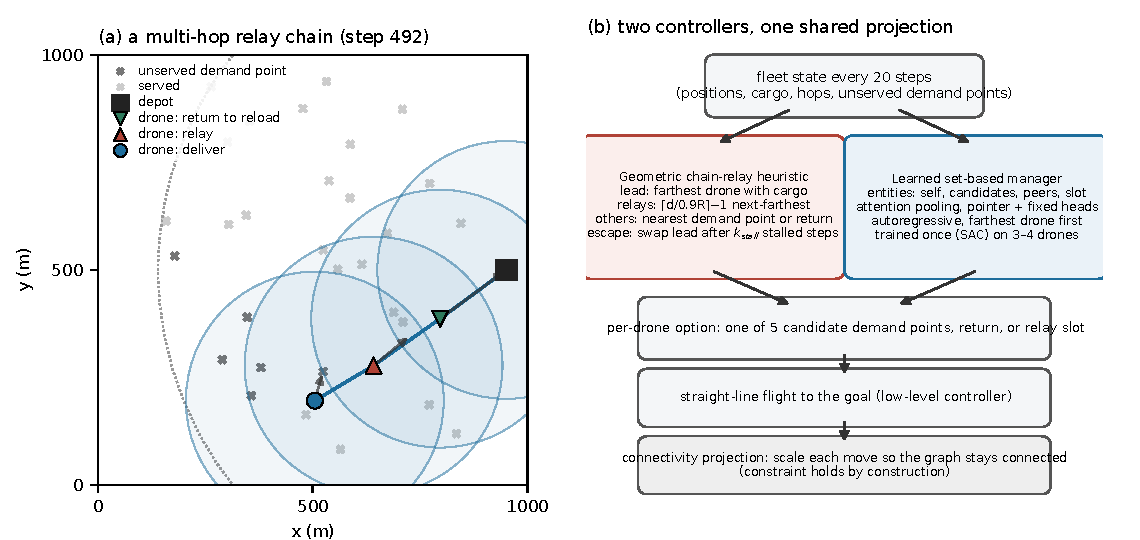
\includegraphics[width=\linewidth]{fig_overview_v5_26_10_17_15.pdf}
\caption{(a) An instance with three drones after 220 steps under the heuristic: the lead drone
(blue circle) heads for a far destination, one drone relays (red triangle) on the segment to the
centre, and one returns to reload; shaded discs are communication ranges and the dotted circle is
the reachable region $0.9NR$. (b) The two controllers emit the same per-drone options and share
the straight-line low-level controller and the connectivity projection.}
\label{fig:overview}
\end{figure}

\subsection{Connectivity-preserving projection}
\label{sec:projection}

A reward penalty for disconnection would punish situations that no action can prevent, for
example a drone that is stationary while unloading and is stranded when a teammate departs. We
therefore enforce the constraint by projection. Given the commanded displacements of all drones,
the projection finds, drone by drone, the largest scaling factor in $[0,1]$ under which the fleet
remains connected, choosing at each round the drone whose restriction leaves the most drones
connected and breaking ties at random so that no anchor drone is starved. A drone whose
displacement is scaled below 10\% is counted as \emph{stalled} for that step. The previous
positions are always connected, so a zero scaling is a valid fallback and the constraint holds by
construction. We refer to this as \emph{radial} projection because the displacement keeps its
direction and loses magnitude; Section~\ref{sec:sensitivity} studies an alternative that keeps the
tangential component.

\subsection{Geometric chain-relay heuristic with deadlock escape}
\label{sec:heuristic}

\paragraph{Assignment rule}
Let $r_i$ be the distance of drone $i$ from the centre. The \emph{lead} is the drone with cargo
that is farthest from the centre. Its target is its nearest unserved destination, at distance
$d$ from the centre; the chain needs $h = \lceil d / (0.9R) \rceil$ hops and therefore
$h - 1$ relays, capped at $N - 1$. The $h-1$ non-lead drones farthest from the centre are
assigned to relay; every other drone with cargo goes to its nearest unserved destination and every
drone without cargo returns to the centre. The rule is evaluated at every decision point and costs
$O(N \log N)$.

\paragraph{Deadlock escape}
The rule is deterministic, so when a geometry stalls the fleet it re-issues the same assignment
and the stall persists: without an escape mechanism the rule completes 62\% of standard instances.
We detect a \emph{partial deadlock} when, among the drones that attempted to move, all but at most
one were stalled by the projection. When a partial deadlock has persisted for $k_{\mathrm{stall}}$
steps, the controller enters an escape phase of $h_{\mathrm{hold}}$ steps during which the lead is
replaced by the next-farthest drone with cargo and the former lead returns to the centre; on the
$n$-th escape of an episode the $n$-th farthest drone becomes the lead, so that repeated escapes
cycle through the fleet. An alternative escape mode, in which every drone except the lead retreats
towards the centre to slacken the chain, is also implemented. The values
$k_{\mathrm{stall}} = 120$, $h_{\mathrm{hold}} = 20$ and the lead-swap mode are selected in
Section~\ref{sec:rq4-heuristic} on seeds disjoint from the evaluation seeds; this setting is used
in every comparison in this paper.

\subsection{Fleet-size-agnostic learned policy}
\label{sec:learned}

\paragraph{Decision structure}
The learned controller is a manager that emits one of the $K = 7$ options for each drone at each
decision point; the low-level controller is the same straight-line flight as the heuristic. A
learned low-level controller was tried in earlier versions and reduced completion to 0--2\%, so it
is not used. Between decision points the environment is a semi-Markov decision process
\cite{sutton1999} and the manager's transitions store the discounted return of the option.

\paragraph{Set-based encoder}
Each drone is encoded from four kinds of entities: its own state (10 features: cargo, distance to
the centre, hop depth, remaining-destination fraction, time, movement ratio, stall indicators,
service timer, cut-vertex indicator), its five candidate destinations (6 features each: distance,
direction, whether a teammate already targets it, distance from the centre, hops required), its
peers ($N-1$ entities of 9 features: relative position, cargo, hop depth and a one-hot of the
peer's current role) and its relay slot (4 features). Distances are normalised by $R$, not by the
map size. Each entity type passes through a two-layer MLP of width 128; the drone's own embedding
is used as the query of two multi-head attention layers that pool the peer set and the candidate
set; the four vectors are concatenated and fused. A pointer head scores the five candidates
against the fused embedding and a fixed head scores \emph{return} and \emph{relay}. Nothing in the
network depends on $N$ or $M$, which is what allows one set of weights to run on fleets it never
saw. Invalid options are masked \cite{huang2022}.

\paragraph{Autoregressive decisions}
Drones are ordered by distance from the centre, farthest first; after each drone's option is
sampled its new role is written into the peer features seen by the drones decided after it. A
formation of one lead and $k$ relays can arise only by coincidence under independent per-drone
sampling, but can be composed deliberately under sequential decisions. The price is $N$ sequential
network calls per decision.

\paragraph{Training}
The manager is trained with discrete soft actor-critic \cite{haarnoja2018}. A twin-Q critic with
attention across drone embeddings outputs per-drone action values whose mean over drones is
regressed on the team return; the actor loss is the standard expectation form. The team reward is
$+10$ per delivery, $+30$ per reload, $-0.01N$ per step and a residual penalty of $-0.1N$ times
the fraction of destinations still unserved; the discount is $\gamma = 0.997$ per step. Three
ingredients matter. (i) \emph{Entropy target annealing}: the conventional target of
$0.6\log n_{\mathrm{valid}}$ keeps the policy too random to hold a multi-step formation, while
that randomness is also the only mechanism by which a deadlocked fleet escapes; annealing the
target linearly from $0.6\log n$ to $0.25\log n$ over the first 400 episodes lowered the
standard-configuration makespan from 1{,}418 to the 900s. (ii) \emph{Rule regularisation}: a
cross-entropy term with weight 2.0 pulls the policy towards the action the heuristic's assignment
rule would take, wherever that action is unmasked. (iii) \emph{Configuration randomisation}:
$N$, $M$ and the depot are resampled every episode. Optimisation uses Adam at $3\times10^{-4}$,
batches of 256 option transitions from a replay buffer of 60{,}000, and Polyak averaging with
$\tau = 0.005$. Checkpoints are scored every 50 episodes on 80 held-out instances with a
3{,}000-step budget by $100f + 40(1 - \bar t/3000)$, where $f$ is the completion rate and $\bar t$
the mean steps, so that one percentage point of completion is worth 75 steps; training stops after
eight evaluations without improvement or at 1{,}000 episodes. One training run takes about 13
hours on a single RTX~5080 when four runs share the GPU.

% =====================================================================================
\section{Experimental Setup}
\label{sec:setup}

\paragraph{Instances and configurations}
Instances are generated from integer seeds; a seed, $N$, $M$ and the depot mode determine the
instance exactly, so two controllers can be run on identical instances. Evaluation seeds are
disjoint from the seeds used for training, for checkpoint selection and for tuning the heuristic.
We evaluate on the standard configuration ($N=4$, $M=50$, fixed depot) and on seven unseen
configurations with random depots: $N/M \in \{3/20, 3/30, 4/80, 5/50, 6/80, 8/150, 10/300\}$.

\paragraph{Baselines}
Besides the two proposed controllers we run a greedy assignment with no relays, two fixed-relay
policies that permanently dedicate one or two drones, and the geometric rule without the escape
mechanism. These establish that the problem is not solved by naive assignment.

\paragraph{Reference model}
For small instances we solve a time-expanded network model with Gurobi~13 \cite{gurobi}: periods
of 10 steps, a lattice with 98.2-metre spacing so that every eight-neighbour move takes one
period, destination and centre nodes added exactly, single-commodity flow for connectivity in
every period and a symmetry-breaking cut. The formulation and its proofs are in a companion
document. Because the lattice restricts where drones may be, the model's optimum is an upper
bound on the continuous optimum and its dual bound is not a bound on the continuous problem; a
certified lower bound through a cell relaxation was attempted and abandoned because the relaxation
inflates a three-hop chain's reach from 900\,m to 1{,}317\,m and returns bounds below the trivial
analytic bound. We therefore call the MILP value a \emph{reference plan}.

\paragraph{Paired protocol}
Averaging only the episodes each method completes favours the method that gives up on hard
instances, and a single long stall moves a 40-rollout mean by over 100 steps. All comparisons
between the two controllers are therefore \emph{paired}: both run on the same instance, the
difference is taken over instances both complete, and we report the median paired difference,
the win--loss count and a Wilcoxon signed-rank $p$-value. Inference samples from the policy;
deterministic argmax inference has the same median but a far heavier tail. The standard
configuration uses 480 rollouts (60 seeds, 8 repetitions, two independent measurement runs),
the $3/30$ and $5/50$ configurations 200 (40 seeds, 5 repetitions) and the remaining
configurations 80 (40 seeds, 2 repetitions). Repetitions differ because the projection's tie
breaking is random. We found 40 rollouts too few to support any claim about tails.

% =====================================================================================
\section{Results}
\label{sec:results}

\subsection{RQ1: Completion under the hard constraint}
\label{sec:rq1}

Connectivity was never violated in any training episode or evaluation rollout, as the projection
guarantees. Table~\ref{tab:completion} reports completion within the 10{,}000-step budget. The
learned policy completes every instance in every configuration. The heuristic with escape
completes 98--100\%; its misses concentrate where drones are plentiful, where a long chain that
is not needed still gets stationed and stalls. Without the escape mechanism the rule completes
61.7\% of standard instances, and the naive baselines complete almost none: the greedy assignment
pulls the fleet apart, and fixed relay counts are wrong for most instances because the number of
relays a destination needs varies with its distance.

\begin{table}[t]
\centering
\caption{Completion within the 10{,}000-step budget. Learning-free baselines on 120 (standard)
or 40 (unseen) rollouts; the two proposed controllers on the paired rollout counts of
Section~\ref{sec:setup}.}
\label{tab:completion}
\small
\begin{tabular}{lrrr}
\toprule
Method & $4/50$ standard & $3/30$ & $5/50$ \\
\midrule
Greedy, no relay & 0\% & 0\% & 25\% \\
One fixed relay & 0\% & 2.5\% & 40\% \\
Two fixed relays & 3.3\% & 52.5\% & 65\% \\
Geometric rule, no escape & 61.7\% & 95\% & 92.5\% \\
Geometric rule + escape (proposed) & 473/480 & 200/200 & 191/200 \\
Learned policy (proposed) & \textbf{480/480} & \textbf{200/200} & \textbf{200/200} \\
\midrule
 & $3/20$ & $4/80$ & $6/80$ \\
Geometric rule + escape (proposed) & 80/80 & 80/80 & 79/80 \\
Learned policy (proposed) & \textbf{80/80} & \textbf{80/80} & \textbf{80/80} \\
\midrule
 & $8/150$ & $10/300$ & \\
Geometric rule + escape (proposed) & 80/80 & 80/80 & \\
Learned policy (proposed) & \textbf{80/80} & \textbf{80/80} & \\
\bottomrule
\end{tabular}
\end{table}

\subsection{RQ2: Distance to the lattice reference plan}
\label{sec:rq2}

\pending{Table~\ref{tab:milp} is being filled from the batch described in
Section~\ref{sec:setup}: ten instances each for $M \in \{4,6,8\}$ and four for $M=10$ with three
drones, time limits of 30 to 120 minutes.} On the instance solved in the earlier study the
reference plan for four destinations is 138 steps after 600 seconds with a 42\% optimality gap
remaining; the heuristic takes 145 and the learned policy a median of 134 over 30 samples
(range 114--287). For six destinations the plan is 176 steps, the heuristic 185 and the learned
median 168 (range 146--484). For ten destinations no feasible plan was found in 90 minutes; the
heuristic takes 244 and the learned median 301. Two points carry over to the full batch. The
heuristic is within 5\% of the reference plan where one exists, so the comparison in RQ3 is
against a strong controller rather than a weak one. The learned policy's median is below the
reference plan on the smallest instances, which is not a contradiction: the plan is restricted to
the lattice and the policy is not.

\begin{table}[t]
\centering
\caption{Lattice MILP reference plans versus the proposed controllers on instances with three
drones (means over instances; makespan in steps). ``Solved'' counts instances for which the solver
returned a feasible plan within the time limit; the gap is Gurobi's remaining optimality gap on
the lattice model. The learned column gives the mean of per-instance medians over 30 samples and
the overall min--max. The ratio column divides the heuristic and the learned median by the
replayed MILP plan on solved instances.}
\label{tab:milp}
\small
\begin{tabular}{l}\toprule \pending{MILP batch in progress} \\ \bottomrule\end{tabular}%

\end{table}

\subsection{RQ3: Performance across environments}
\label{sec:rq3}

\paragraph{Fleet size divides the configuration space}
Table~\ref{tab:paired} and Figure~\ref{fig:regime} give the paired comparison across the eight
configurations. With three drones the heuristic is faster by 39 and 30 steps in paired median with 20 and
30 destinations. With four drones the two controllers tie: on the standard configuration the
median paired difference over 480 rollouts is $+2$ steps with 234 wins against 239
($p = 0.52$), and on $4/80$ the learned policy is 38 steps faster. With five or more drones the
learned policy is faster and the margin grows monotonically with the fleet, from 62 steps at five
drones to 178 at ten. The boundary therefore lies at four drones. An earlier measurement against
the heuristic's pre-tuning escape parameters gave the same picture ($+40$, $+0$, $-54$, $-170$ on
$3/30$, $4/50$, $5/50$ and $10/300$), so the boundary does not depend on the tuning.

\begin{table}[t]
\centering
\caption{Paired comparison on identical instances. Positive differences mean the learned policy
is slower than the heuristic. $p$ from the Wilcoxon signed-rank test on both-completed pairs.}
\label{tab:paired}
\small
\begin{tabular}{lrrrrrr}
\toprule
$N/M$ & rollouts & complete h/l & median heuristic / learned & paired median & win--loss & $p$ \\
\midrule
3/20 & 80 & 80/80 & 366 / 422 & $+36$ & 20--60 & $<10^{-4}$ \\
3/30 & 200 & 200/200 & 572 / 617 & $+40$ & 73--127 & $<10^{-4}$ \\
4/50 (standard) & 480 & 473/480 & 868 / 872 & $+0$ & 236--236 & 0.885 \\
4/80 & 80 & 79/80 & 1,109 / 1,048 & $-24$ & 49--30 & 0.026 \\
5/50 & 200 & 190/200 & 570 / 534 & $-54$ & 141--45 & $<10^{-4}$ \\
6/80 & 80 & 79/80 & 732 / 606 & $-126$ & 70--9 & $<10^{-4}$ \\
8/150 & 80 & 80/80 & 916 / 740 & $-148$ & 75--5 & $<10^{-4}$ \\
10/300 & 80 & 80/80 & 1,201 / 1,022 & $-170$ & 76--4 & $<10^{-4}$ \\
\bottomrule
\end{tabular}%

\end{table}

\begin{figure}[t]
\centering
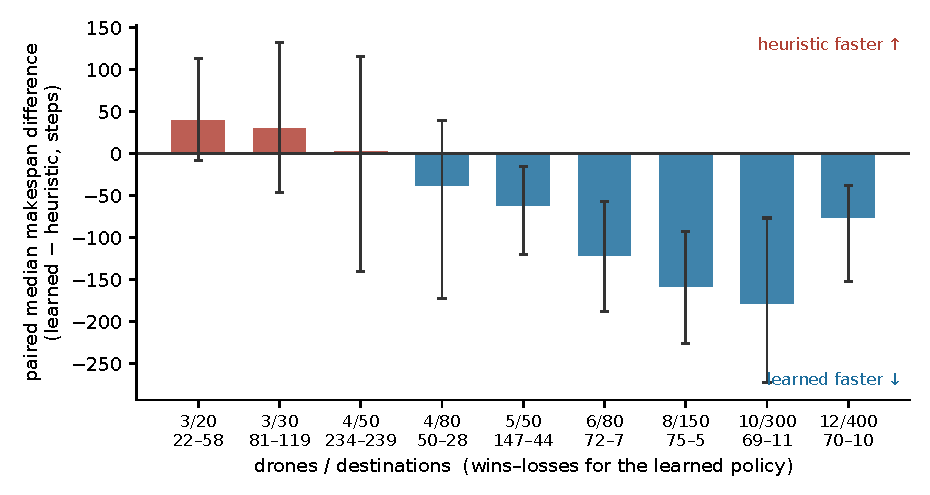
\includegraphics[width=0.8\linewidth]{fig_regime_v5_26_10_17_15.pdf}
\caption{Paired median makespan difference (learned minus heuristic) by configuration, with the
interquartile range of the paired differences as error bars and the learned policy's wins--losses
under each label. Negative values favour the learned policy; the boundary lies at four drones.}
\label{fig:regime}
\end{figure}

Figure~\ref{fig:cdf} shows the full distributions on the three main configurations: with three
drones the heuristic's curve lies to the left, with four the curves coincide, and with five the
learned policy's curve lies to the left and reaches completion earlier.

\begin{figure}[t]
\centering
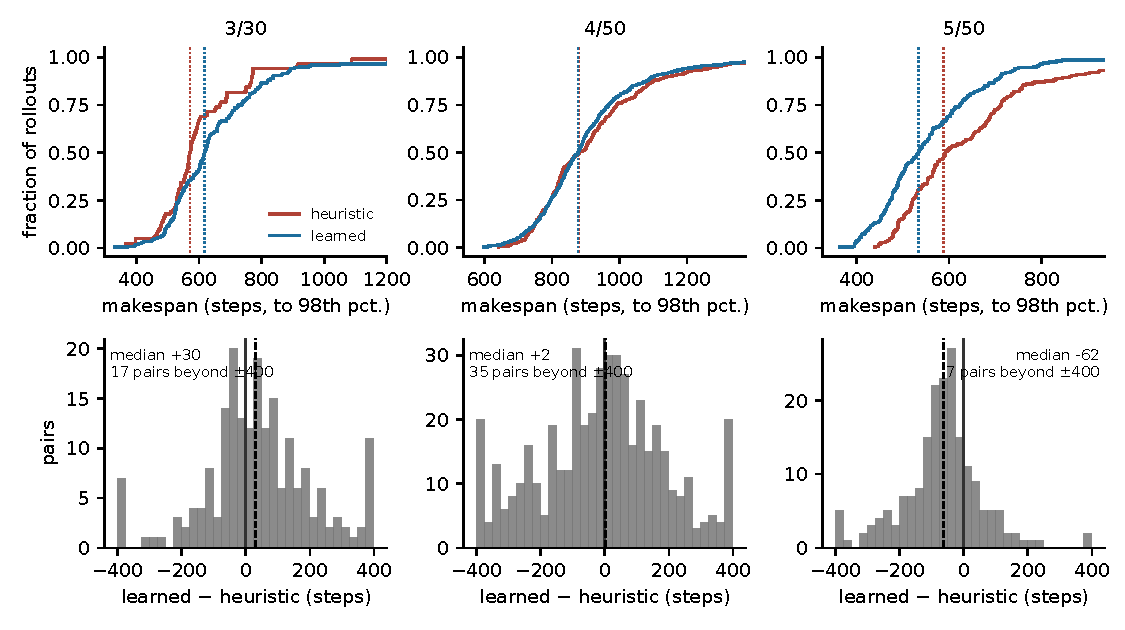
\includegraphics[width=\linewidth]{fig_cdf_v5_26_10_17_15.pdf}
\caption{Top: cumulative distribution of makespan on $3/30$, $4/50$ and $5/50$ (dotted lines
mark medians; axes cut at the 98th percentile). Bottom: distribution of the paired difference on
both-completed instances, clipped to $\pm400$ steps with the number of clipped pairs noted.}
\label{fig:cdf}
\end{figure}

\paragraph{Tails follow the same split}
Where drones are scarce the learned policy's worst case is three to four times the heuristic's
(maximum 5{,}395 versus 1{,}447 steps on $3/30$); where they are plentiful it is lighter (1{,}101
versus 1{,}734 on $5/50$, 1{,}365 versus 1{,}753 on $10/300$). On the standard configuration over
480 rollouts against the pre-tuning heuristic the learned policy exceeded 1{,}500 steps five times
and the heuristic fourteen times.

\paragraph{Mechanism}
The two controllers differ in one decision. On $3/30$ the heuristic stations 1.39 relays on
average and the learned policy 0.78; the learned fleet therefore spends 27\% of drone-steps stalled
by the projection against 8\% for the heuristic. Overriding only the learned policy's relay
assignment with the heuristic's, at inference, recovers the full 44-step gap; matching only the
\emph{number} of relays recovers 14 steps of median but removes the tail (maximum from 4{,}904 to
1{,}083). The identity of the relaying drone drives the median and the count drives the tail. The
information needed to make the heuristic's choice is present in the learned policy's observation:
a two-layer classifier predicts the heuristic's relay assignment from the 41 observed features with
85\% accuracy, and behaviour cloning of the full rule reaches 95\% on relay decisions. When drones
are plentiful the opposite happens: the heuristic keeps stationing a chain that the geometry no
longer needs, while the learned policy exploits the slack and, with its sampled inference, escapes
the stalls that the deterministic rule repeats; this is also where the heuristic loses its few
completions.

\paragraph{Why the scarce-fleet deficit resists policy-side fixes}
\label{sec:negative}
Table~\ref{tab:negative} lists ten interventions, each trained with four or two seeds under the
same recipe and evaluated with the same paired protocol, that attempt to make the learned policy
relay like the heuristic when drones are scarce. None improves the $3/30$ median and several hurt
the configurations where the learned policy wins. The pattern is informative. Adding reward for
relaying turns the means into the end: the policy relays for its own sake and $5/50$ reverses from
$-54$ to $+60$. Every route to per-drone credit is blocked for a different reason: a joint-action
critic inherits the variance of a sampled teammate action in its target; a monotonic mixing
network either diverges when its weights are free or collapses to the mean when they are floored;
a sequential single-agent reformulation removes the decomposition but leaves an undiscounted
credit chain with no contraction. Initialising the policy by behaviour cloning of the rule, with
95\% relay accuracy, is erased within 400 episodes: once the actor is updated, relay usage falls to
the level of a randomly initialised policy within 50 episodes and stays there. A penalty on the
bottleneck destination's estimated arrival makes the policy reduce the \emph{average} rather than
the maximum. We conclude that, within this policy structure and objective, under-relaying is the
learner's fixed point, not an artefact of credit, information or initialisation.

\begin{table}[t]
\centering
\caption{Interventions that did not remove the scarce-fleet deficit. Paired median against the
heuristic (positive is slower); the proposed recipe is the reference row. These runs were
evaluated against the heuristic with its pre-tuning escape parameters ($k_{\mathrm{stall}}=60$,
$h_{\mathrm{hold}}=40$), so the column values are comparable to the reference row of this table
but not numerically identical to Table~\ref{tab:paired}, which uses the tuned heuristic.}
\label{tab:negative}
\small
\begin{tabular}{lrrrl}
\toprule
Intervention & $3/30$ & $5/50$ & $4/50$ & Mechanism of failure \\
\midrule
Proposed recipe (reference) & $+40$ & $-54$ & $+0$ & --- \\
Relay-weighted rule regularisation & $+54$, $+56$ & $-44$, $-19$ & $+41$, $+54$ & relay-specific regularisation harms \\
Per-drone relay credit & $+36$ to $+82$ & $+60$ to $+106$ & $+39$ to $+131$ & relaying becomes the goal \\
Checkpoint selection on $3/30$ (8 seeds) & $+58$ & $-42$ & $+10$ & improves only the standard config.\\
Zero-sum credit redistribution & $+91$, $+126$ & $+98$, $+172$ & $+146$, $+180$ & same, larger \\
Joint-action critic & $+89$ & $-27$ & $+58$ & target variance from sampled teammates \\
Near-first decision order & $+46$, $+100$ & $-43$, $-38$ & $+4$, $+106$ & order is not the cause \\
Re-decision on stall (learned) & $+82$, $+95$ & $-38$, $-34$ & $+17$, $+55$ & irregular option lengths \\
Monotonic mixing critic & $+145$ & $+5$ & $+139$ & divergence vs.\ credit on one axis \\
Sequential single-agent credit & $+142$ & $+17$ & $+116$ & no contraction within a decision \\
Behaviour-cloning initialisation & $+42$ to $+69$ & $-42$ to $-20$ & $-4$ to $+40$ & erased within 400 episodes \\
Bottleneck-arrival penalty & $+105$ & $-8$ & $+81$ & reduces the mean, not the maximum \\
\bottomrule
\end{tabular}
\end{table}

\paragraph{Sensitivity to the connectivity enforcement model}
\label{sec:sensitivity}
The projection of Section~\ref{sec:projection} scales a blocked displacement along its own
direction, so a drone pulling on the chain effectively stops. We implemented an alternative that
clamps the target position to the nearest point of the communication disc around the binding
neighbour, which removes only the outward component and keeps the tangential one (a drone can
still circle at constant range). Both controllers use the same projection in each comparison, and
connectivity is still never violated. These measurements predate the heuristic tuning of Section~\ref{sec:rq4-heuristic} and use
$k_{\mathrm{stall}}=60$, $h_{\mathrm{hold}}=40$ for both projections, so they are internally
consistent. Evaluating the same learned weights under the sliding projection without retraining
reduces the $3/30$ deficit from $+40$ to $+21$; retraining four
seeds under it gives $+15$ to $+48$ (mean $+28$) and lowers the learned fleet's stall ratio from
0.27 to 0.17--0.22, with completion still 100\%. The heuristic gains little with three drones
(median 570 to 571) but gains more than the learned policy with four (866 to 812 against 879 to
850), so the standard-configuration tie becomes $+26$ in its favour. We therefore keep the radial
projection as the primary model and report this as a sensitivity result: about half of the
three-drone deficit is a property of how the constraint is enforced rather than of the learner.

\paragraph{Communication radius}
Both controllers were run without retraining at $R = 250$\,m and $R = 350$\,m
(Table~\ref{tab:range}, Figure~\ref{fig:range}); the learned policy normalises distances by $R$,
and the instance generator rescales the reachable region $0.9NR$ with $R$, so both controllers see
the same instances at each radius. Completion transfers: the learned policy completes every
instance at both radii, while the heuristic loses 18 of 200 instances on $5/50$ at the shorter
radius. Speed shows two effects. The first is the regime shift seen with fleet size: at
$R=250$\,m a destination needs more hops, the fleet is effectively scarcer, and every
configuration moves towards the heuristic ($+77$ on $3/30$, $+68$ on $4/50$, and the $5/50$
advantage shrinks to a tie at $-16$, $p=0.33$); at $R=350$\,m the fleet is effectively more
plentiful and the learned policy is faster already with four drones ($-40$ on $4/50$). The second
is a training-radius effect: on $3/30$ and $5/50$ the learned policy's margin is best at the
radius it was trained on and worse on both sides ($+30$ at 300\,m against $+77$ and $+52$;
$-62$ against $-16$ and $-42$), so the normalisation by $R$ transfers completion but not the full
speed. The regime variable is therefore the chain demand, the hops a destination needs relative
to the drones available, rather than the fleet size alone, and a deployment at a radius far from
the training radius should retrain or at least re-evaluate the boundary.

\begin{figure}[t]
\centering
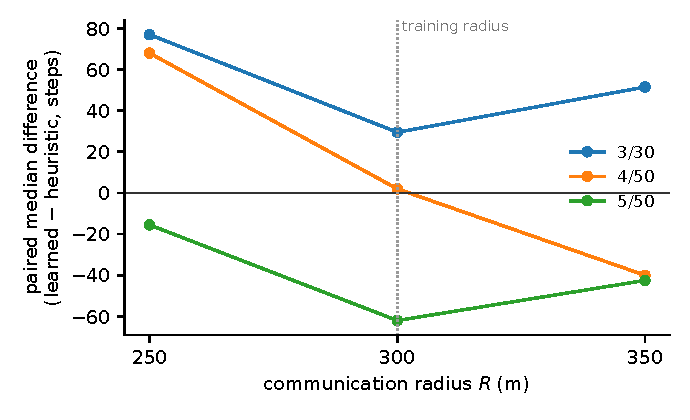
\includegraphics[width=0.6\linewidth]{fig_range_v5_26_10_17_15.pdf}
\caption{Paired median difference against the communication radius without retraining
(training radius 300\,m, dotted). A shorter radius moves every configuration towards the
heuristic; a longer radius helps the learned policy on $4/50$ but not beyond its training-radius
margin on $3/30$ and $5/50$.}
\label{fig:range}
\end{figure}

\begin{table}[t]
\centering
\caption{Transfer to other communication radii without retraining. Cells give completions
(heuristic/learned) and the paired median difference with win--loss and $p$; $R=300$\,m is the
training radius.}
\label{tab:range}
\small
\begin{tabular}{lrrr}
\toprule
$N/M$ & $R=250$\,m & $R=300$\,m & $R=350$\,m \\
\midrule
3/30 & --- & 200/200 \,/\, $+40$ (73--127, $<10^{-4}$) & --- \\
4/50 & --- & 473/480 \,/\, $+0$ (236--236, 0.885) & --- \\
5/50 & --- & 190/200 \,/\, $-54$ (141--45, $<10^{-4}$) & --- \\
\bottomrule
\end{tabular}%

\end{table}

\subsection{RQ4: Are the components necessary?}
\label{sec:rq4}

\paragraph{Heuristic}
\label{sec:rq4-heuristic}
Table~\ref{tab:heur-ablation} grids $k_{\mathrm{stall}} \in \{30,60,90,120\}$,
$h_{\mathrm{hold}} \in \{20,40,80\}$ and the two escape modes, plus no escape, on $3/30$,
$4/50$ and $5/50$ with 40 tuning seeds each, and ranks settings by total completions first and
the sum of median makespans second; this criterion was fixed before the measurement. The escape
mechanism is necessary: without it the rule completes 26 of 40 standard instances. The mode
matters more than the timing: every lead-swap setting completes 117--120 of 120 instances, while
retreat settings complete 100--117 because slackening the chain does not change the assignment
that caused the stall. Within the lead-swap family the medians differ by at most 40 steps summed
over three configurations, which is within the noise of 40 instances; the selected setting
($k_{\mathrm{stall}}=120$, $h_{\mathrm{hold}}=20$) is the only one that completes all 120 and
also has the lowest median sum. The adaptive relay count is necessary as well: fixing one or two
relays completes 0--65\% (Table~\ref{tab:completion}).

\begin{table}[t]
\centering
\caption{Heuristic ablation on tuning seeds disjoint from the evaluation seeds (40 instances per
configuration). Cells give completed instances and the median makespan over completed instances;
the last column sums completions over the three configurations.}
\label{tab:heur-ablation}
\small
\begin{tabular}{llrrrr}
\toprule
mode & $k_{\mathrm{stall}}$ / $h_{\mathrm{hold}}$ & $3/30$ & $4/50$ & $5/50$ & completions \\
\midrule
none & --- & 39/40 \,/\, 559 (0.228) & 25/40 \,/\, 817 (0.258) & 38/40 \,/\, 602 (0.093) & 102/120 \\
lead swap & 30 / 20 & 40/40 \,/\, 557 (0.121) & 39/40 \,/\, 853 (0.130) & 40/40 \,/\, 625 (0.928) & 119/120 \\
lead swap & 30 / 40 & 40/40 \,/\, 562 (0.673) & 40/40 \,/\, 867 (0.775) & 40/40 \,/\, 606 (0.247) & 120/120 \\
lead swap & 30 / 80 & 40/40 \,/\, 567 (0.158) & 39/40 \,/\, 844 (0.754) & 39/40 \,/\, 614 (0.404) & 118/120 \\
lead swap & 60 / 20 & 40/40 \,/\, 557 (0.599) & 39/40 \,/\, 849 (0.780) & 40/40 \,/\, 600 (0.791) & 119/120 \\
lead swap & 60 / 40 & 40/40 \,/\, 554 (0.497) & 39/40 \,/\, 852 (0.807) & 40/40 \,/\, 625 (0.944) & 119/120 \\
lead swap & 60 / 80 & 40/40 \,/\, 556 (0.359) & 39/40 \,/\, 863 (0.788) & 39/40 \,/\, 632 (0.675) & 118/120 \\
lead swap & 90 / 20 & 40/40 \,/\, 566 (0.206) & 39/40 \,/\, 871 (0.908) & 40/40 \,/\, 599 (0.375) & 119/120 \\
lead swap & 90 / 40 & 40/40 \,/\, 559 (0.473) & 40/40 \,/\, 856 (0.674) & 37/40 \,/\, 634 (0.844) & 117/120 \\
lead swap & 90 / 80 & 40/40 \,/\, 563 (0.786) & 39/40 \,/\, 858 (0.149) & 39/40 \,/\, 629 (0.615) & 118/120 \\
\textbf{lead swap} & \textbf{120 / 20} & 40/40 \,/\, 561 & 40/40 \,/\, 867 & 40/40 \,/\, 620 & \textbf{120/120} \\
lead swap & 120 / 40 & 40/40 \,/\, 557 (0.757) & 39/40 \,/\, 878 (0.685) & 40/40 \,/\, 624 (0.979) & 119/120 \\
lead swap & 120 / 80 & 40/40 \,/\, 562 (0.687) & 38/40 \,/\, 829 (0.546) & 39/40 \,/\, 626 (0.850) & 117/120 \\
retreat & 30 / 20 & 37/40 \,/\, 559 (0.350) & 35/40 \,/\, 836 (0.185) & 40/40 \,/\, 632 (0.528) & 112/120 \\
retreat & 30 / 40 & 39/40 \,/\, 556 (0.079) & 29/40 \,/\, 832 (0.284) & 39/40 \,/\, 621 (0.157) & 107/120 \\
retreat & 30 / 80 & 38/40 \,/\, 561 (0.754) & 26/40 \,/\, 804 (0.443) & 37/40 \,/\, 584 (0.368) & 101/120 \\
retreat & 60 / 20 & 39/40 \,/\, 556 (0.866) & 38/40 \,/\, 847 (0.215) & 38/40 \,/\, 603 (0.759) & 115/120 \\
retreat & 60 / 40 & 39/40 \,/\, 559 (0.875) & 39/40 \,/\, 823 (0.485) & 39/40 \,/\, 624 (0.459) & 117/120 \\
retreat & 60 / 80 & 39/40 \,/\, 563 (0.991) & 26/40 \,/\, 795 (0.236) & 40/40 \,/\, 635 (0.490) & 105/120 \\
retreat & 90 / 20 & 39/40 \,/\, 566 (0.512) & 38/40 \,/\, 822 (0.058) & 40/40 \,/\, 642 (0.773) & 117/120 \\
retreat & 90 / 40 & 39/40 \,/\, 566 (0.180) & 39/40 \,/\, 852 (0.634) & 39/40 \,/\, 618 (0.615) & 117/120 \\
retreat & 90 / 80 & 39/40 \,/\, 562 (0.665) & 36/40 \,/\, 830 (0.578) & 37/40 \,/\, 598 (0.354) & 112/120 \\
retreat & 120 / 20 & 39/40 \,/\, 556 (0.645) & 37/40 \,/\, 863 (0.327) & 38/40 \,/\, 614 (0.460) & 114/120 \\
retreat & 120 / 40 & 39/40 \,/\, 560 (0.757) & 37/40 \,/\, 831 (0.451) & 38/40 \,/\, 628 (0.602) & 114/120 \\
retreat & 120 / 80 & 39/40 \,/\, 561 (0.191) & 38/40 \,/\, 854 (0.815) & 37/40 \,/\, 627 (0.308) & 114/120 \\
\bottomrule
\end{tabular}%

\end{table}

\paragraph{Learned policy}
Table~\ref{tab:ablation} removes one ingredient at a time, retrains two seeds and evaluates on the
three main configurations; values are makespan differences from the proposed recipe. Four
independent trainings of the same recipe span 919 to 979 steps on the standard configuration, so
a two-seed mean is meaningful only beyond 70--80 steps. Rule regularisation and configuration
randomisation are necessary; entropy annealing is the single largest contributor on the standard
configuration; autoregressive decisions help with four drones and more; the residual penalty is
neutral. A manager with a fixed-size MLP encoder instead of the set encoder, trained in an earlier
version on the standard configuration only, completed 38\% of standard instances and could not be
run on other fleet sizes at all.

\begin{table}[t]
\centering
\caption{Ablation of the learned policy: makespan difference from the proposed recipe over
completed episodes, two seeds. Positive means the removed component was needed. Differences below
70--80 steps are within seed variance.}
\label{tab:ablation}
\small
\begin{tabular}{lrrr}
\toprule
Removed component & $4/50$ & $3/30$ & $5/50$ \\
\midrule
Rule regularisation & $+320$ & $+408$ & $+92$ \\
Configuration randomisation & $-44$ & $+646$ & $+68$ \\
Entropy target annealing & $+128$ & $+19$ & $+61$ \\
Autoregressive decisions & $+94$ & $-46$ & $+33$ \\
Residual penalty & $-28$ & $-37$ & $+8$ \\
\bottomrule
\end{tabular}
\end{table}

\subsection{Inference cost}
\label{sec:cost}

Table~\ref{tab:latency} gives the latency of one manager decision on a CPU. The heuristic costs
0.05--0.12\,ms; the learned policy 1.3--2.5\,ms without autoregression and 2.7--7.4\,ms with it,
growing linearly with the fleet because each drone is a sequential network call. Over a 900-step
episode the learned policy's cumulative decision time is 0.16\,s. The lattice MILP takes 600 to
5{,}400 seconds on instances with four to ten destinations and does not return a plan for ten.

\begin{table}[t]
\centering
\caption{Latency of one manager decision (milliseconds, CPU) and the cumulative decision time of
a 900-step episode.}
\label{tab:latency}
\small
\begin{tabular}{lrrrrr}
\toprule
Controller & $N=3$ & $N=4$ & $N=6$ & $N=8$ & 900 steps \\
\midrule
Geometric rule + escape & 0.05 & 0.08 & 0.10 & 0.12 & 0.003\,s \\
Learned, independent decisions & 1.27 & 1.52 & 1.94 & 2.45 & 0.069\,s \\
Learned, autoregressive (proposed) & 2.70 & 3.52 & 5.32 & 7.35 & 0.158\,s \\
\bottomrule
\end{tabular}
\end{table}

% =====================================================================================
\section{Discussion}
\label{sec:discussion}

\paragraph{Deployment}
The two controllers are complementary and the boundary is sharp, so a fleet operator can choose
by fleet size: the heuristic with three drones, the learned policy with five or more, where it is
both faster and more reliable; with four the two tie and the learned policy completes more. Both decide in milliseconds and both keep the fleet connected by
construction.

\paragraph{What the negative results mean}
Ten interventions that change how the learner is credited, informed, initialised or rewarded leave
the scarce-fleet deficit in place, and a change to the environment's enforcement model removes
half of it. The deficit is therefore best understood as an interaction between the learner's
fixed point under this objective and the geometry of the constraint, not as a shortcoming that
more training or a better critic would fix. For a practitioner the actionable consequence is the
one above: pick the controller by regime.

\paragraph{Limitations}
The learned policy was trained at a single communication radius; it transfers to radii of 250 and
350\,m in completion but its speed ranking against the heuristic shifts with the radius
(Section~\ref{sec:rq3}), and radii outside this range were not tested. The environment is planar, ignores
wind, battery and collisions, and uses a disc communication model; real links are not discs. The
MILP reference is a lattice restriction with a remaining optimality gap, not an exact optimum. The
heuristic's novelty lies in the escape mechanism and the adaptive relay count rather than in the
chain geometry itself.

\paragraph{Methodological notes}
Three practices mattered for the conclusions. Completed-episode averages favour the controller that
gives up, so comparisons must be paired. Forty rollouts cannot support claims about tails; several
of our own interim conclusions reversed when the sample grew. And a pre-check that uses a different
metric from the final judgement will pass interventions that the final judgement rejects.

% =====================================================================================
\section{Conclusion}
\label{sec:conclusion}

We proposed two controllers for connectivity-constrained drone delivery, a geometric chain-relay
heuristic with deadlock escape and a fleet-size-agnostic learned policy, both acting through a
projection that keeps the fleet connected at every step. Under a paired protocol across fleets of
three to ten drones the learned policy completes every instance and is faster by 38 to 178 steps
once more than four drones are available, while the heuristic is faster by 30--39 steps with
three. The scarce-fleet deficit is one decision, which drone relays; it resists ten policy-side
interventions and halves when the enforcement model is changed. Both controllers are three orders
of magnitude faster than exact optimisation on a lattice, which stops returning plans at ten
destinations. The natural next step is a policy whose output is a team assignment rather than a
set of per-drone options, so that the relay identity becomes a coordinate the critic can value
directly.

\section*{Acknowledgements}
\pending{To be added.}

\section*{Data and code availability}
Code, trained weights, instance generators and the paired-comparison records are available at
\url{https://github.com/koptimizer/relay_drone_network}.

\bibliographystyle{elsarticle-num}
\bibliography{paper_v5_26_10_17_15}

\end{document}
